\documentclass[10pt]{article}
\usepackage{graphicx}
\usepackage{float}
\usepackage{amsmath}
\usepackage{amsfonts}
\usepackage[brazilian]{babel}
\usepackage[utf8]{inputenc}
\usepackage{csquotes}
\usepackage[usenames,dvipsnames,svgnames,table]{xcolor}
%\usepackage{docmute}
\usepackage{array}
\usepackage{multicol}
\usepackage{listings}
\usepackage{geometry}
\usepackage[T1]{fontenc}

\newcommand{\fromeng}[1]{\footnote{do inglês: \textit{#1}}}
\newcommand{\tit}[1]{\textit{#1}}
\newcommand{\tbf}[1]{\textbf{#1}}
\newcommand{\ttt}[1]{\texttt{#1}}

\newcolumntype{C}[1]{>{\centering\let\newline\\\arraybackslash\hspace{0pt}}m{#1}}

\lstset{%
	language=R,
	basicstyle=\scriptsize\ttfamily,
	commentstyle=\ttfamily\color{gray},
	numbers=left,
	numberstyle=\ttfamily\color{blue}\footnotesize,
	stringstyle=\ttfamily\color{olive}\footnotesize,
	stepnumber=1,
	numbersep=5pt,
	backgroundcolor=\color{white},
	showspaces=false,
	showstringspaces=false,
	showtabs=false,
	frame=single,
	tabsize=2,
	captionpos=b,
	breaklines=true,
	breakatwhitespace=false,
	%title=\lstname,
	escapeinside={},
	keywordstyle={},
	morekeywords={}
}

\begin{document}

\begin{titlepage}
	\centering
	{\scshape\Large MC884/MO444 - Aprendizado de Máquina\par}
	\vspace{1.5cm}
    {\huge\bfseries k-means\par}
	\vspace{1cm}
	{\itshape Erik de Godoy Perillo - RA135582\par}
	\vfill
	Universidade Estadual de Campinas
	\vfill
	{\large \today\par}
\end{titlepage}

\newpage

\section{Introdução}
O objetivo do trabalho era explorar o algoritmo de \tit{k-means} e suas
métricas de desempenho.

\subsection{Implementação}
A linguagem de implementação escolhida foi o R.
Todo o código utilizado no relatório encontra-se na seção~\ref{code}.
Ao longo do documento, linhas do código serão citadas para referência no mesmo.
A função \ttt{main} (linha 18 da seção~\ref{code}) executa tudo que é
requisitado no enunciado, mostrando os resultados.

\section{Metodologia}
Os parâmetros para o \tit{k-means} encontram-se na linha 11 da seção~\ref{code}.
Para métrica interna, foi selecionado o \ttt{dunn2}, que mede
a razão entre a mínima dissimilaridade média entre clusters e a máxima
dissimilaridade média intra-clusters.
Para métrica externa, foi selecionado o \tit{corrected rand}.
A seleção dos melhores \ttt{k} para as duas métricas é feita no \tit{loop}
da linha 39 e as métricas são plotadas na linha 76.

\section{Resultados}
Para a métrica interna, o melhor \ttt{k} foi 2, com $dunn2 = 2.739$.
Para a externa, o melhor \ttt{k} foi 4, com $rand = 0.258$.
A saída da execução do código encontra-se na seção~\ref{output}.
Os \tit{plots} encontram-se abaixo.
\newpage
\begin{figure}[H]
    \centering
    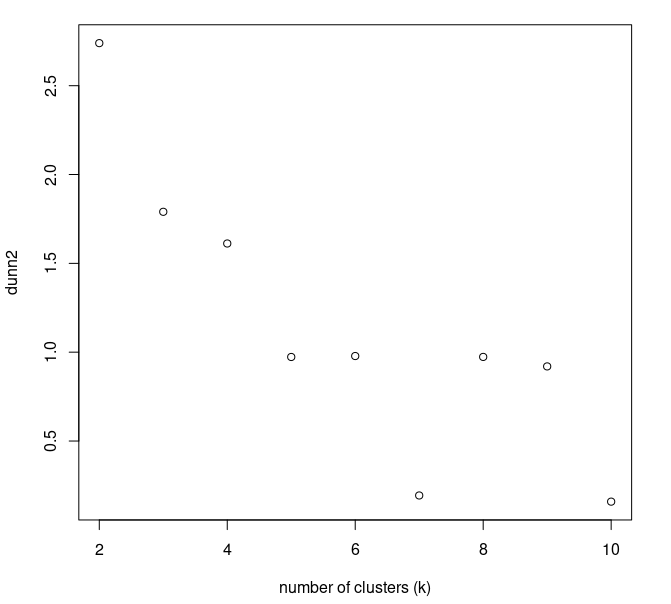
\includegraphics[width=0.6\linewidth]{dunn2.png}
    \caption{Métricas internas para cada k}
\end{figure}

\begin{figure}[H]
    \centering
    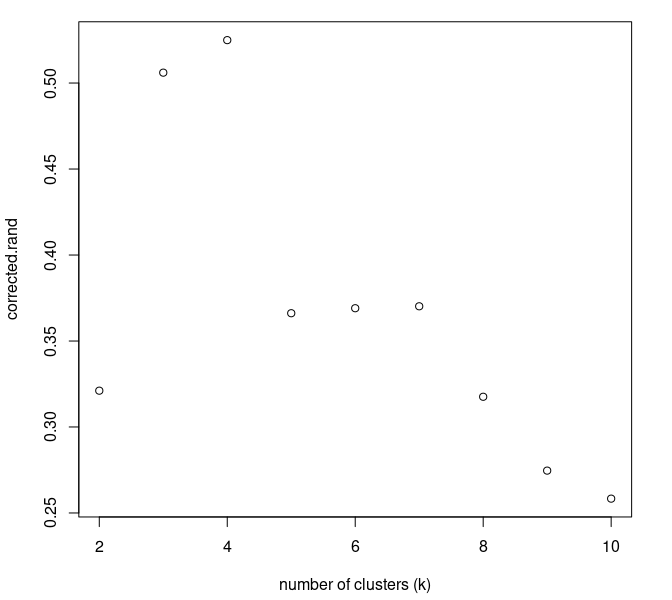
\includegraphics[width=0.6\linewidth]{rand.png}
    \caption{Métricas externas para cada k}
\end{figure}

\newpage
\section{Código-fonte}
\label{code}
\lstinputlisting{../ch_4.r}

\newpage

\section{Saída do código}
\label{output}
\lstinputlisting{../res.txt}

\end{document}
